\documentclass[11pt, a4paper]{article}
\usepackage[utf8]{inputenc}
\usepackage[T1]{fontenc}
\usepackage[a4paper, margin=2.5cm]{geometry}
\usepackage[english]{babel}

\usepackage{amsmath}
\usepackage{amssymb}
\usepackage{booktabs}
\usepackage{tabularx}
\usepackage{fancyhdr}
\usepackage{xcolor}
\usepackage{graphicx}
\usepackage{float}
\usepackage{hyperref}

\hypersetup{
    colorlinks=true,
    linkcolor=blue,
    urlcolor=blue,
    pdftitle={Microstates and Macroscopic Thermodynamics of a Binary System}
}

% Page Header and Footer setup
\pagestyle{fancy}
\fancyhf{}
\rhead{\small Statistical Physics Lab 1}
\lhead{\small Microstates of a System of Coins}
\lfoot{\small UC3M}
\rfoot{\small Page \thepage}
\renewcommand{\headrulewidth}{0.4pt}
\renewcommand{\footrulewidth}{0.4pt}

\fancypagestyle{plain}{%
  \fancyhf{}%
  \lfoot{\small UC3M}%
  \rfoot{\small Page \thepage}%
  \renewcommand{\headrulewidth}{0pt}%
  \renewcommand{\footrulewidth}{0.4pt}%
}

% All numerical results are generated by `python main.py`
% Auto-generated by main.py - do not edit by hand.
\newcommand{\NsevenTotal}{\ensuremath{128}}
\newcommand{\Workers}{\ensuremath{16}}
\newcommand{\NmaxGen}{\ensuremath{29.9}}
\newcommand{\NmaxVec}{\ensuremath{36.2}}
\newcommand{\SlopeGen}{\ensuremath{1.045}}
\newcommand{\SlopeVec}{\ensuremath{0.920}}
\newcommand{\CostGen}{\ensuremath{307.1}}
\newcommand{\CostVec}{\ensuremath{3.83}}
\newcommand{\NverifyVal}{\ensuremath{36}}
\newcommand{\TverifyVal}{\ensuremath{99}}
\newcommand{\OmegaPeakTwenty}{\ensuremath{1.848\times10^{5}}}
\newcommand{\PPeakTwenty}{\ensuremath{0.1762}}
\newcommand{\OmegaPeakFifty}{\ensuremath{1.264\times10^{14}}}
\newcommand{\PPeakFifty}{\ensuremath{0.1123}}
\newcommand{\OmegaPeakEighty}{\ensuremath{1.075\times10^{23}}}
\newcommand{\PPeakEighty}{\ensuremath{0.0889}}
\newcommand{\OmegaPeakHundred}{\ensuremath{1.009\times10^{29}}}
\newcommand{\PPeakHundred}{\ensuremath{0.0796}}
\newcommand{\LimTotal}{\ensuremath{1024}}
\newcommand{\LimFact}{\ensuremath{171}}
\newcommand{\LimCentral}{\ensuremath{1030}}
\newcommand{\FloatMax}{\ensuremath{1.80\times10^{308}}}
\newcommand{\MCtrials}{\ensuremath{100\,000}}
\newcommand{\MCchi}{\ensuremath{41.3}}
\newcommand{\MCdof}{\ensuremath{42}}
\newcommand{\MCmean}{\ensuremath{49.991}}
\newcommand{\MCmeanErr}{\ensuremath{0.016}}
\newcommand{\NIAdigits}{\ensuremath{29, 04, 04, 60}}
\newcommand{\Mexact}{\ensuremath{24.25}}
\newcommand{\Mval}{\ensuremath{24}}
\newcommand{\Nval}{\ensuremath{124}}
\newcommand{\Nhalf}{\ensuremath{62}}
\newcommand{\NisOdd}{even}
\newcommand{\HalfNote}{Since $N$ is even, the equal split $N/2=62$ is a valid macrostate.}
\newcommand{\TotalStates}{\ensuremath{2.127\times10^{37}}}
\newcommand{\PthirtyHeads}{\ensuremath{2.46\times10^{-9}}}
\newcommand{\OmegaThirty}{\ensuremath{5.222\times10^{28}}}
\newcommand{\PhalfHeads}{\ensuremath{0.07151}}
\newcommand{\OmegaHalf}{\ensuremath{1.521\times10^{36}}}
\newcommand{\PtenHeads}{\ensuremath{0.9411}}
\newcommand{\PtwentyTails}{\ensuremath{0.999796}}
\newcommand{\PtwentyTailsComp}{\ensuremath{2.04\times10^{-4}}}
\newcommand{\SigmaN}{\ensuremath{5.6}}
\newcommand{\TenInSigma}{\ensuremath{1.8}}
\newcommand{\TwentyInSigma}{\ensuremath{3.6}}
\newcommand{\ThirtyInSigma}{\ensuremath{5.7}}
\newcommand{\OutsideTenPct}{\ensuremath{5.9}}
\newcommand{\dSAfrom}{\ensuremath{87}}
\newcommand{\dSAto}{\ensuremath{62}}
\newcommand{\dSA}{\ensuremath{10.285}}
\newcommand{\dSASI}{\ensuremath{1.42\times10^{-22}}}
\newcommand{\dSAratio}{\ensuremath{2.93\times10^{4}}}
\newcommand{\dSAabs}{\ensuremath{10.3}}
\newcommand{\dSBfrom}{\ensuremath{72}}
\newcommand{\dSBto}{\ensuremath{62}}
\newcommand{\dSB}{\ensuremath{1.607}}
\newcommand{\dSBSI}{\ensuremath{2.22\times10^{-23}}}
\newcommand{\dSBratio}{\ensuremath{4.99}}
\newcommand{\dSBabs}{\ensuremath{1.6}}
\newcommand{\dSCfrom}{\ensuremath{62}}
\newcommand{\dSCto}{\ensuremath{20}}
\newcommand{\dSC}{\ensuremath{-30.862}}
\newcommand{\dSCSI}{\ensuremath{-4.26\times10^{-22}}}
\newcommand{\dSCratio}{\ensuremath{3.95\times10^{-14}}}
\newcommand{\dSCabs}{\ensuremath{30.9}}
\newcommand{\PeightHeads}{\ensuremath{5.18\times10^{-26}}}
\newcommand{\WaitEightS}{\ensuremath{1.93\times10^{25}}}
\newcommand{\WaitEightYears}{\ensuremath{6.12\times10^{17}}}
\newcommand{\WaitEightUniverse}{\ensuremath{4.44\times10^{7}}}
\newcommand{\MPlus}{\ensuremath{34}}
\newcommand{\PPlus}{\ensuremath{1.61\times10^{-7}}}
\newcommand{\RatioPlus}{\ensuremath{4.43\times10^{5}}}
\newcommand{\MMinus}{\ensuremath{14}}
\newcommand{\PMinus}{\ensuremath{5.11\times10^{-20}}}
\newcommand{\RatioMinus}{\ensuremath{1.40\times10^{18}}}
\newcommand{\TLwidth}{\ensuremath{3.16\times10^{-12}}}
\newcommand{\TLsigma}{\ensuremath{1.58\times10^{11}}}
\newcommand{\TLPhalf}{\ensuremath{2.52\times10^{-12}}}
\newcommand{\TLlogRatio}{\ensuremath{-8.69\times10^{16}}}
\newcommand{\TLdSkB}{\ensuremath{-2.00\times10^{17}}}
\newcommand{\TLdSSI}{\ensuremath{-2.76\times10^{-6}}}
\newcommand{\TLeps}{\ensuremath{1\times10^{-10}}}
\newcommand{\TLz}{\ensuremath{63}}
\newcommand{\TLtail}{\ensuremath{3.25\times10^{-871}}}
\newcommand{\TLPeight}{\ensuremath{10^{-3.01\times10^{22}}}}
\newcommand{\GaussErrHundred}{\ensuremath{0.25}}


\newcommand{\kB}{k_{\mathrm{B}}}
% Expandable input for generated table rows (\input is not expandable in a tabular)
\makeatletter\newcommand{\tabinput}[1]{\@@input #1 }\makeatother

\title{\textbf{Microstates and Macroscopic Thermodynamics of a Binary System}\\
\large Statistical Physics --- Laboratory Practice 1}

\author{\textbf{Group X}\\[0.5em]
Rocío Fernández Jover (NIA: 100523129, GitHub: \texttt{@user1})\\
J. Cantillana (NIA: 100496704, GitHub: \texttt{@jcantillana04})\\
Olivia (NIA: 100XXXXXX, GitHub: \texttt{@olivia614})\\
Author 4 (NIA: 100XXXXXX, GitHub: \texttt{@user4})\\
\\[0.3em]
\small Department of Physics, Universidad Carlos III de Madrid}

\date{\today}

\begin{document}

\maketitle

\begin{abstract}
\noindent We study a system of $N$ independent unbiased coins as an exact model of a two-state assembly. A modular Python package enumerates all $2^N$ microstates by bitwise encoding, computes the multiplicities $\Omega(N,k)$ exactly and in log-space, and evaluates probabilities and Boltzmann entropies. Full enumeration is limited by its $\mathcal{O}(2^N)$ cost: the largest system fully enumerated within five minutes of wall-clock time is $N=\NverifyVal$. For the assigned system of $N=\Nval$ coins the equal-split macrostate has probability $\PhalfHeads$, while $\PtenHeads$ of all outcomes lie within $\pm10$ heads of it. Entropy differences between macrostates are of order $10\,\kB$, i.e.\ $10^{-22}$\,J/K. As $N\to10^{23}$ the relative width of the distribution falls to $\TLwidth$, and macroscopic decreases of entropy become unobservable. This is the statistical content of the Second Law.
\end{abstract}

\vspace{0.5em}
\noindent \textbf{Repository:} \url{https://github.com/olivia614/StatisticalPhysicsLab1}

\vspace{1em}

%==========================================================================
\section{Introduction \& Objectives}
%==========================================================================
A microstate of $N$ distinguishable coins is the ordered list of the face of every coin. A macrostate is specified only by the number of heads $k$. Every one of the $2^N$ microstates is equally likely for unbiased coins. The multiplicity of a macrostate is the number of ways to choose which $k$ coins show heads:
\begin{equation}
\Omega(N,k) = \binom{N}{k} = \frac{N!}{k!\,(N-k)!}, \qquad \sum_{k=0}^{N}\Omega(N,k)=(1+1)^N = 2^N .
\label{eq:omega}
\end{equation}
The probability of a macrostate and its Boltzmann entropy are therefore
\begin{equation}
P(N,k) = \frac{\Omega(N,k)}{2^{N}}, \qquad S(N,k) = \kB \ln \Omega(N,k).
\label{eq:PS}
\end{equation}
The objectives are: (i) to enumerate microstates and determine how far brute force can go; (ii) to compute and plot $\Omega(N,k)$ for $N=20$--$100$; (iii) to evaluate probabilities and entropy changes for $N=100+M$; and (iv) to extrapolate to $N\sim10^{23}$ and interpret the Second Law statistically.

%==========================================================================
\section{Methodology \& Collaborative Workflow}
%==========================================================================

\subsection{Environment \& Reproducibility}
The environment is a Conda environment (\texttt{statphys\_lab1}, Python 3.11, NumPy, SciPy, Matplotlib, pytest) specified in \texttt{environment.yml}. Running \texttt{python main.py} regenerates every figure in \texttt{report/figures/} and every number in this report (\texttt{report/results.tex}). The timing study runs with \texttt{python main.py --benchmark}.

\subsection{Version Control \& Repository Architecture}
Development followed a feature-branch workflow on GitHub, with direct pushes to \texttt{main} disabled and pull requests reviewed by at least one teammate. The code is organised as:
\begin{itemize}
    \item \texttt{src/microstates.py}: bitwise enumeration (generator and chunked NumPy versions), benchmark utilities.
    \item \texttt{src/combinatorics.py}: exact big-integer and log-gamma binomial coefficients, floating-point limits.
    \item \texttt{src/thermodynamics.py}: probabilities, entropy, waiting times, Gaussian limit, Monte Carlo tosses.
    \item \texttt{tests/}: 68 \texttt{pytest} unit tests checking every routine against \texttt{math.comb} and analytical identities.
    \item \texttt{main.py}: orchestrates all calculations; \texttt{report/}: \LaTeX{} source and figures.
\end{itemize}

\subsection{Numerical uncertainty}
All combinatorial quantities are exact integers or are computed in double precision with relative error below $10^{-12}$; this is verified by unit tests against exact integer arithmetic. They are quoted to three or four significant figures. The only measured quantities are wall-clock times. These are reported as the mean $\pm$ sample standard deviation of three repetitions on a 16-thread laptop CPU.

%==========================================================================
\section{Computational Analysis of Microstates}
%==========================================================================

\subsection{Enumeration for $N=7$}
Each microstate is encoded as an integer $s\in[0,2^N)$ whose bit $i$ is 1 if coin $i$ shows heads. Iterating over \texttt{range(1 << N)} with a Python generator visits every microstate exactly once in $\mathcal{O}(1)$ memory. The macrostate is the population count of $s$ (\texttt{s.bit\_count()}). Table~\ref{tab:macrostate_7} summarises the $\NsevenTotal$ outcomes for $N=7$; the complete listing is given in Appendix~\ref{app:n7}. The counts reproduce row 7 of Pascal's triangle and sum to $2^7$.

\begin{table}[H]
\centering
\caption{Macrostates of $N=7$ coins: multiplicity $\Omega(7,k)$ obtained by enumeration, and probability $P_k$.}
\label{tab:macrostate_7}
\begin{tabular}{cccrc}
\toprule
\textbf{Heads $k$} & \textbf{Tails $7-k$} & \textbf{Example microstate} & $\mathbf{\Omega(7,k)}$ & $\mathbf{P_k}$ \\
\midrule
\tabinput{tables/n7_summary.tex}
\midrule
 & & \textbf{Total} & 128 & 1 \\
\bottomrule
\end{tabular}
\end{table}

\subsection{Largest $N$ for full enumeration}
Two implementations were timed (Table~\ref{tab:performance}, Fig.~\ref{fig:benchmark}). The first is the pure-Python generator. The second splits $[0,2^N)$ into blocks of $2^{22}$ consecutive integers; for each block it computes popcounts in compiled NumPy code (\texttt{np.bitwise\_count}) and distributes the blocks over $\Workers$ processes. Both genuinely visit every microstate; no combinatorial shortcut is used. A least-squares fit of $\log_2 t = a + bN$ over the four largest $N$ of each method (smaller $N$ are dominated by fixed overheads) gives slopes $b=\SlopeGen$ (generator) and $b=\SlopeVec$ (vectorised), to be compared with $b=1$ for a doubling of the cost per added coin. Because the timings are noisy over a short range of $N$, the extrapolation instead imposes the theoretical scaling $t=c\,2^N$. The cost per microstate $c$ is taken as the median of $t/2^N$, giving $c=\CostGen$\,ns (generator) and $c=\CostVec$\,ns (vectorised, wall-clock over all processes). Extrapolating to $t=300$\,s gives $N_{\max}\approx\NmaxGen$ for the generator and $N_{\max}\approx\NmaxVec$ for the parallel version. The extrapolation was checked with direct runs (stars in Fig.~\ref{fig:benchmark}). The largest $N$ enumerated within the limit is $N_{\max}=\NverifyVal$, which took $\TverifyVal$\,s; its histogram reproduced $\Omega(N,\lfloor N/2\rfloor)$ exactly. Timings depend on the hardware and on background load, with a run-to-run scatter of about 5--15\%.

\begin{table}[H]
\centering
\caption{Wall-clock time (mean $\pm$ s.d., 3 runs) for building the full histogram of $2^N$ microstates. Memory is the peak traced allocation per process (generator / one vectorised worker); the last rows are single verification runs.}
\label{tab:performance}
\begin{tabular}{ccccc}
\toprule
$\mathbf{N}$ & $\mathbf{2^N}$ & \textbf{Generator (s)} & \textbf{Vectorised (s)} & \textbf{Mem.\ gen\,/\,vec (MB)} \\
\midrule
\tabinput{tables/benchmark.tex}
\bottomrule
\end{tabular}
\end{table}

\begin{figure}[!htb]
\centering
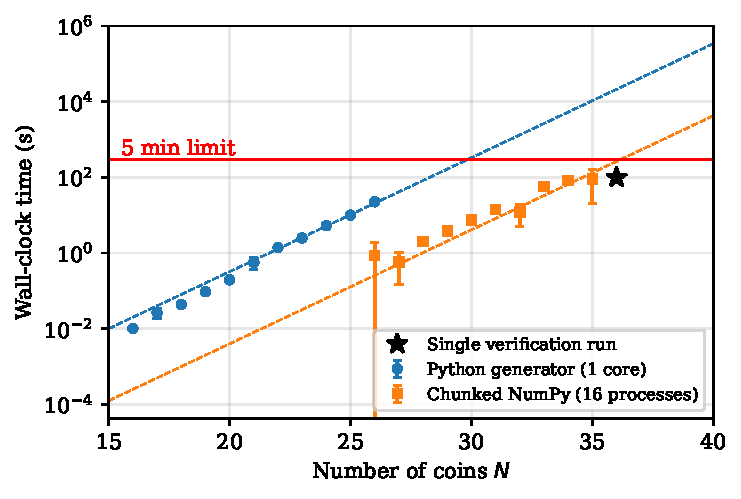
\includegraphics[width=0.62\linewidth]{figures/fig_benchmark.pdf}
\caption{Enumeration time versus $N$ (log scale). Dashed lines are the exponential fits; the horizontal line is the five-minute limit.}
\label{fig:benchmark}
\end{figure}

\paragraph{Why larger $N$ cannot be reached.}
The limit is the exponential size of the state space, not the implementation. Each additional coin doubles the number of microstates and hence the run time. At $\sim1$\,ns per state even an ideal code needs $2^{40}\,\text{ns}\approx18$\,min for $N=40$ and about 36\,years for $N=60$. Storing the states instead of generating them would need $8\times2^N$ bytes, i.e.\ 8\,GB at $N=30$ and 8\,TB at $N=40$; generators avoid this. Writing the list (as required for $N=7$) costs $N\cdot2^N$ characters, which is already 32\,GB at $N=30$. Fixed-width integer encoding also caps the vectorised method at $N=63$.

\subsection{Macrostate distributions ($N=20,50,80,100$)}
For these $N$, listing microstates is impossible, so $\Omega(N,k)$ is evaluated directly. Factorials are never formed: the code uses exact Python integers via the Pascal recurrence $\Omega(N,k)=\Omega(N-1,k-1)+\Omega(N-1,k)$ for the plots, and log-space evaluation
\begin{equation}
\ln \Omega(N,k) = \ln \Gamma(N+1) - \ln \Gamma(k+1) - \ln \Gamma(N-k+1)
\label{eq:lgamma}
\end{equation}
for probabilities. Figure~\ref{fig:distributions} shows the results. The peak multiplicity grows from $\OmegaPeakTwenty$ ($N=20$) to $\OmegaPeakHundred$ ($N=100$), while the peak probability falls from $\PPeakTwenty$ to $\PPeakHundred$. The distribution broadens in $k$ as $\sqrt N$, but it narrows relative to $N$.

\begin{figure}[!htb]
\centering
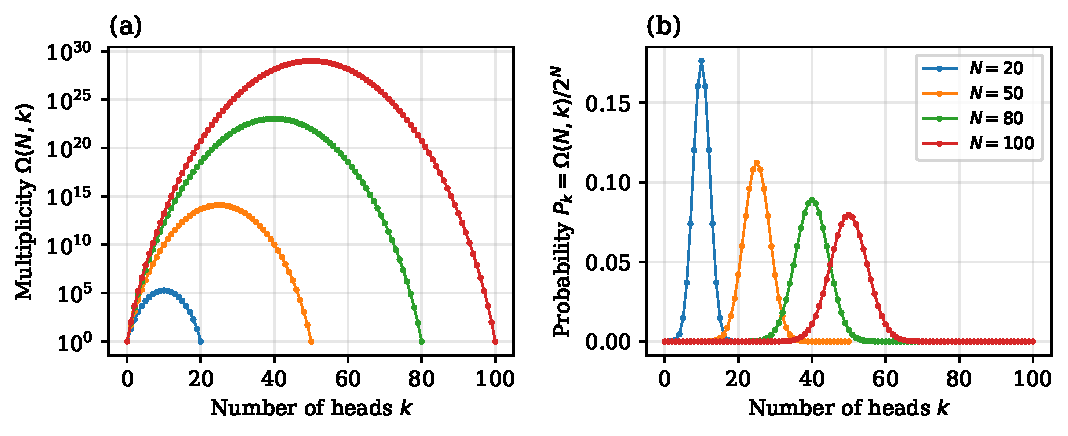
\includegraphics[width=0.92\linewidth]{figures/fig_distributions.pdf}
\caption{(a) Number of microstates $\Omega(N,k)$ with $k$ heads (log scale). (b) Normalised probability $P_k=\Omega(N,k)/2^N$.}
\label{fig:distributions}
\end{figure}

As a check, $\MCtrials$ simulated tosses of $N=100$ coins (Appendix~\ref{app:mc}, Fig.~\ref{fig:simulation}) give mean $\langle k\rangle=\MCmean\pm\MCmeanErr$ (expected 50). Comparing the simulated histogram with Eq.~\eqref{eq:PS} gives $\chi^2=\MCchi$ for $\MCdof$ degrees of freedom, so the two agree within counting uncertainty.
\paragraph{Maximum $N$ that can be calculated.}
There is no hard limit with the methods above; only the representation limits it.
\begin{itemize}
\item In IEEE double precision, the total $2^N$ overflows ($>\FloatMax$) at $N=\LimTotal$.
\item A naive $N!/[k!(N-k)!]$ already fails at $N=\LimFact$.
\item The largest multiplicity $\Omega(N,N/2)$ overflows at $N=\LimCentral$.
\end{itemize}
Arbitrary-precision integers remove the overflow, at a cost that grows with the number of digits ($\approx0.3N$). Eq.~\eqref{eq:lgamma} has no limit at all: the unit tests evaluate it at $N=10^{23}$, where it agrees with Stirling's formula to $10^{-12}$.

\subsection{Thermodynamic limit ($N \rightarrow 10^{23}$)}
Applying Stirling's formula $\ln N!\approx N\ln N-N+\tfrac12\ln(2\pi N)$ to Eq.~\eqref{eq:omega} and expanding around $k=N/2$ to second order in $\delta=k-N/2$ gives the de~Moivre--Laplace result
\begin{equation}
P(N,k)\simeq\sqrt{\frac{2}{\pi N}}\exp\!\left[-\frac{2(k-N/2)^2}{N}\right],\qquad
\mu=\frac N2,\quad \sigma=\frac{\sqrt N}{2},\quad \frac{\sigma}{\mu}=\frac1{\sqrt N}.
\label{eq:gauss}
\end{equation}
The approximation is already accurate to $\GaussErrHundred\%$ at the peak for $N=100$. For $N=10^{23}$ the absolute width $\sigma=\TLsigma$ is large, but the relative width is $\sigma/\mu=\TLwidth$ (Fig.~\ref{fig:thermo}).
\begin{itemize}
\item The fraction of heads is $1/2$ to eleven significant figures.
\item A deviation $|k/N-\tfrac12|>\TLeps$ is a $\TLz\sigma$ event, with probability $\TLtail$.
\item Even a $0.1\%$ deviation ($k/N=0.501$) is suppressed by a factor $10^{\TLlogRatio}$.
\end{itemize}
The distribution is then effectively a delta function: the system is always found in the most probable macrostate, which is the equilibrium state.

\begin{figure}[!htb]
\centering
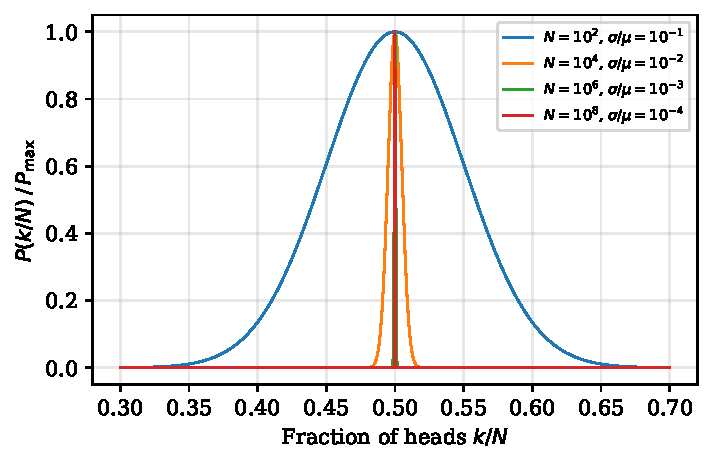
\includegraphics[width=0.58\linewidth]{figures/fig_thermo_limit.pdf}
\caption{Probability distribution versus the fraction of heads $k/N$ for increasing $N$ (Eq.~\ref{eq:gauss}). The relative width scales as $N^{-1/2}$.}
\label{fig:thermo}
\end{figure}

%==========================================================================
\section{Probabilities, Entropy, and Thermodynamics}
%==========================================================================

\subsection{Parameter assignment}
$M$ is the arithmetic mean of the last two digits of the team members' NIAs ($\NIAdigits$), which is $\Mexact$, rounded to $M=\Mval$. Hence $N=100+M=\Nval$ coins, with $2^N=\TotalStates$ microstates. \HalfNote

\subsection{Probability and entropy analysis}
All probabilities follow from Eq.~\eqref{eq:PS}. Range probabilities are sums over $k$, evaluated with a log-sum-exp to avoid underflow. Entropy changes for a transition $k_1\to k_2$ are
\begin{equation}
\frac{\Delta S}{\kB}=\ln\frac{\Omega(N,k_2)}{\Omega(N,k_1)},\qquad \kB=1.380649\times10^{-23}\ \mathrm{J/K}.
\end{equation}
Results are collected in Table~\ref{tab:entropy} and illustrated in Fig.~\ref{fig:prob}.

\begin{table}[H]
\centering
\caption{Probabilities and entropy changes for $N=\Nval$ coins (questions 1--9).}
\label{tab:entropy}
\begin{tabularx}{\linewidth}{@{}lX r@{}}
\toprule
\textbf{Question} & \textbf{Quantity} & \textbf{Result} \\
\midrule
1 & $P(k=30)$, with $\Omega=\OmegaThirty$ & $\PthirtyHeads$ \\
2 & $P(k=\Nhalf)$, with $\Omega=\OmegaHalf$ & $\PhalfHeads$ \\
3 & $P(\Nhalf-10\le k\le\Nhalf+10)$ heads & $\PtenHeads$ \\
4 & $P(\Nhalf-20\le N-k\le\Nhalf+20)$ tails & $\PtwentyTails$ \\
\midrule
5 & $\Delta S$: $k=\dSAfrom\to\dSAto$ heads ($\Omega$ ratio $\dSAratio$) & $\dSA\,\kB=\dSASI$ J/K \\
6 & $\Delta S$: $k=\dSBfrom\to\dSBto$ heads ($\Omega$ ratio $\dSBratio$) & $\dSB\,\kB=\dSBSI$ J/K \\
7 & $\Delta S$: $k=\dSCfrom\to\dSCto$ heads ($\Omega$ ratio $\dSCratio$) & $\dSC\,\kB=\dSCSI$ J/K \\
\midrule
8 & $P(k=8)$; mean wait at 1 toss/s & $\PeightHeads$;\ \ $\WaitEightS$ s \\
9 & $P(\Nhalf)/P(M+10=\MPlus)$ & $\RatioPlus$ \\
  & $P(\Nhalf)/P(M-10=\MMinus)$ & $\RatioMinus$ \\
\bottomrule
\end{tabularx}
\end{table}

\begin{figure}[!htb]
\centering
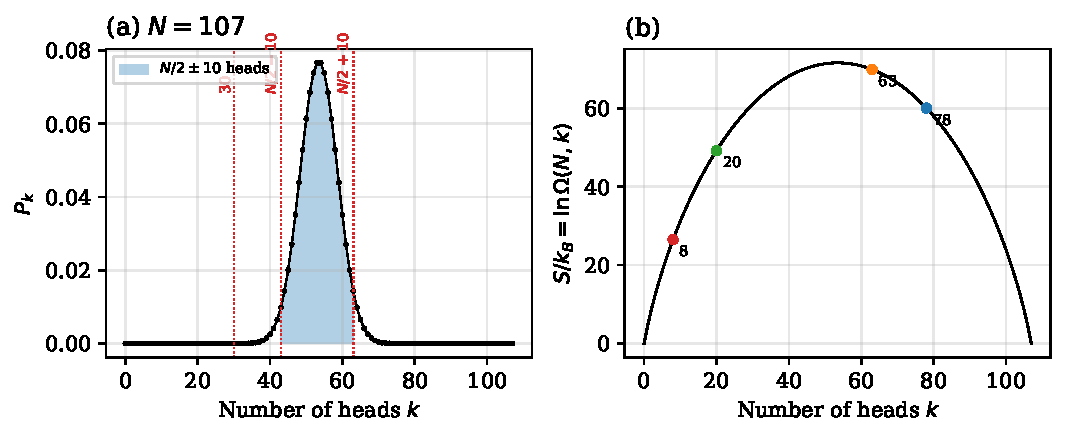
\includegraphics[width=0.92\linewidth]{figures/fig_probabilities.pdf}
\caption{(a) $P_k$ for $N=\Nval$; the shaded band is $\Nhalf\pm10$ heads and dotted lines mark $k=30$ and $M\pm10$. (b) Entropy $S/\kB=\ln\Omega$; points mark the states used in questions 5--8.}
\label{fig:prob}
\end{figure}

\paragraph{Discussion of questions 1--4.}
Although $\Nhalf$ heads is the single most probable outcome, its probability is only $\PhalfHeads$ because there are $\Nval+1$ possible macrostates. Ranges matter more: about $\sigma=\sqrt N/2\approx\SigmaN$, so $\pm10$ heads covers $\approx\TenInSigma\sigma$ and holds $\PtenHeads$ of the probability. The $\pm20$-tails window ($\approx\TwentyInSigma\sigma$) misses only $\PtwentyTailsComp$. By contrast, $k=30$ lies $\ThirtyInSigma\sigma$ below the mean and has probability $\PthirtyHeads$.

\paragraph{Question 8.}
Each toss is an independent trial with success probability $p=P(N,8)$. The number of tosses until the first success is therefore geometric, with mean $1/p$. At one toss per second the expected wait is $\WaitEightS$\,s, which is $\WaitEightYears$ years or $\WaitEightUniverse$ times the age of the Universe.

\paragraph{Question 9.}
The equal split is $\RatioPlus$ times more likely than $M+10=\MPlus$ heads, and $\RatioMinus$ times more likely than $M-10=\MMinus$ heads.

\subsection{Second Law of Thermodynamics interpretation (question 10)}
None of these results contradicts the Second Law, because in statistical mechanics the Second Law is a statement about probabilities, not a strict prohibition. The microscopic dynamics (re-tossing coins) are reversible, and every microstate is equally likely, including the ``ordered'' ones. A transition from $k=\Nhalf$ to $k=20$ lowers the entropy by $\dSC\,\kB$. It is not forbidden; it is simply $\Omega(\Nhalf)/\Omega(20)=e^{\,\dSCabs}$ times rarer than the reverse. For $N=\Nval$, fluctuations of a few $\kB$ (questions 5--6) do occur: about $\OutsideTenPct\%$ of tosses fall outside $\Nhalf\pm10$. These fluctuations are visible only because $N$ is small. The Second Law is the statement that the macrostate with maximum $\Omega$ (maximum $S$) overwhelmingly dominates, so a spontaneous evolution almost always goes towards higher entropy.

\subsection{The limit $N\gg1$ (question 11)}
For $N\sim10^{23}$, Eq.~\eqref{eq:gauss} and the log-space routines give:
\begin{itemize}
\item \textbf{Fixed $k$ (30 heads, 8 heads, $M\pm10$).} The probability is $\sim2^{-N}$. For example, $P(k=8)=\TLPeight$, so the waiting time and the likelihood ratios of question 9 become $10^{\sim3\times10^{22}}$. These events never happen.
\item \textbf{$P(N/2)$} $=\sqrt{2/\pi N}=\TLPhalf\to0$, and so does any window of fixed width $\pm10$ or $\pm20$: that width is negligible compared with $\sigma=\TLsigma$. What tends to 1 is the probability of any \emph{relative} window $|k/N-\tfrac12|<\varepsilon$.
\item \textbf{Entropy.} Fixed offsets ($N/2+25\to N/2$) give $\Delta S\simeq2\delta^2\kB/N\approx10^{-20}\kB\to0$. Macroscopic offsets ($k/N=0.501\to0.5$) give $\Delta S=\TLdSkB\,\kB$ in magnitude, i.e.\ about $\TLdSSI$\,J/K, which is a measurable thermodynamic entropy.
\end{itemize}
In the thermodynamic limit, therefore, the probabilistic statement of question 10 becomes a deterministic law. Entropy-decreasing macroscopic fluctuations have probabilities $\exp(-\Delta S/\kB)\sim10^{-10^{17}}$, and the Second Law holds without exception in practice.

%==========================================================================
\section{Conclusion}
%==========================================================================
Bitwise enumeration confirms $\Omega(N,k)=\binom Nk$ directly, but the $2^N$ cost limits it to $N=\NverifyVal$ in five minutes, even with vectorisation and parallelism. Log-space combinatorics removes all overflow limits and allows exact statements for $N=\Nval$ and asymptotic ones for $N=10^{23}$. The binomial distribution narrows relative to $N$ as $N^{-1/2}$. Entropy-lowering fluctuations, observable for $N\sim10^2$, become unobservable for macroscopic $N$. This is the statistical origin of the Second Law of Thermodynamics.

\appendix
%==========================================================================
\section{AI Collaboration \& Audit Statement}
%==========================================================================
Following Phase~3 of the course guidelines, AI assistance (Anthropic Claude Code, model Claude Opus~5.5) was used for planning, code generation and drafting this report. Every prompt, the files generated and the team's modifications are logged in \texttt{AI\_STATEMENT.md} at the repository root. The planning transcript is in \texttt{docs/ai\_plans/}. Verification consisted of:
\begin{enumerate}
\item 68 \texttt{pytest} unit tests comparing every AI-written routine with exact integer arithmetic (\texttt{math.comb}), identities ($\sum_k\Omega=2^N$, symmetry) and published values ($\Omega(100,50)\approx1.009\times10^{29}$).
\item An independent Monte Carlo cross-check of the distribution ($\chi^2/\text{dof}=\MCchi/\MCdof$).
\item Re-derivation by the team of all formulas in Sections~3--4.
\end{enumerate}
Issues found during the audit are documented in \texttt{AI\_STATEMENT.md}: a floating-point edge case in the overflow-limit routine, and a LAPACK/MKL crash in the Conda environment.

%==========================================================================
\section{Monte Carlo cross-check}
\label{app:mc}
%==========================================================================
Tossing $N=100$ coins $\MCtrials$ times with NumPy's pseudo-random generator (seed 2026) reproduces the exact distribution within the Poisson counting uncertainty $\sqrt{n_k}$ of each bin.

\begin{figure}[h]
\centering
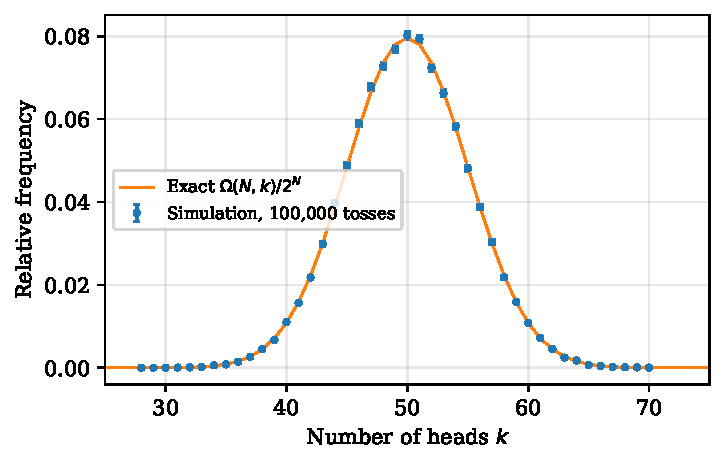
\includegraphics[width=0.58\linewidth]{figures/fig_simulation.pdf}
\caption{Monte Carlo relative frequencies for $N=100$ (error bars: Poisson $\sqrt{n_k}$) against the exact distribution.}
\label{fig:simulation}
\end{figure}

%==========================================================================
\section{Complete list of microstates for $N=7$}
\label{app:n7}
%==========================================================================
\begin{center}
\small
\begin{tabularx}{\linewidth}{@{}l>{\raggedright\arraybackslash}X@{}}
\toprule
\textbf{Macrostate ($\Omega$)} & \textbf{Microstates} \\
\midrule
\tabinput{tables/n7_full.tex}
\bottomrule
\end{tabularx}
\end{center}

%==========================================================================
\section{Core algorithms}
%==========================================================================
\begin{verbatim}
def iter_microstates(n):              # src/microstates.py
    state, total = 0, 1 << n          # 2**n microstates, O(1) memory
    while state < total:
        yield state
        state += 1

counts[state.bit_count()] += 1        # macrostate = number of set bits

# chunked version: popcount a block of 2**22 states in compiled code
states = offsets + np.uint64(block << chunk_bits)
counts += np.bincount(np.bitwise_count(states), minlength=n + 1)

def log_binom(n, k):                  # src/combinatorics.py, Eq. (3)
    return gammaln(n + 1) - gammaln(k + 1) - gammaln(n - k + 1)
\end{verbatim}

\end{document}
